\section{開発した学習ツールについて}

\subsection{開発の目的}
これらの問題を受け,学習者がCUDに配慮した工夫を項目ごとに実践でき,自動で別色覚での見え方と評価・改善案を表示する学習ツールの開発を行った.

\subsection{対象とする学習者}
CUDに関する講習等では,色覚異常やCUDに関する説明を受けた後に,色覚異常の見え方やCUDに配慮したデザインを体験する場面がある.
そのため,色覚異常やCUDについてある程度学習している者を対象とした.

\subsection{想定している利用方法}
本学習ツールは,実際の資料作成の際にCUDに配慮した工夫をどのように取り入れるかを学習させることを目的としている.
そのため,CUDの講習等でCUDに配慮した工夫の取り入れ方を教育する場合や,CUDについて学習した者が実際に資料作成を行う前段階として,本学習ツールを利用することを想定している.

\subsection{利用環境}
本学習ツールは,iPadやPCでの使用を想定して,Web上で動作するよう開発した.


\clearpage

\subsection{学習の流れ}
例として,第1部1項目目の内容である文字の強調における配色について学習する際の学習の流れについて説明する.
この例における学習画面の遷移を図\ref{fig:map}に示す.

この項目では,まず文字の強調に使用する色を選択する.

①選択肢から色を選択すると,下の文の一部の色が変化する.
赤が選択されている場合は,文の一部が赤色になっている.

②評価ボタンが押されると,評価画面が表示される.
評価画面で別色覚での見え方と評価・改善案が表示される.

③この項目において,赤,緑,青は一部の色覚では黒との区別がつきづらい色に見えるため,文字の強調には適さない.
適さない色を選択した場合は,色を再選択する.

④橙,黄緑,空色は赤,緑,青に比べどの色覚でも黒との区別がつきやすい色となっている.
適した色を選択した場合,他の適する選択肢を試していない場合は別の色を再選択する.

⑤適する色を全て試した場合は,次の項目に進む.

この一連の流れを項目ごとに行い,CUDに配慮した工夫を一つ一つ学習する.

\begin{figure}[h]
\begin{center}
 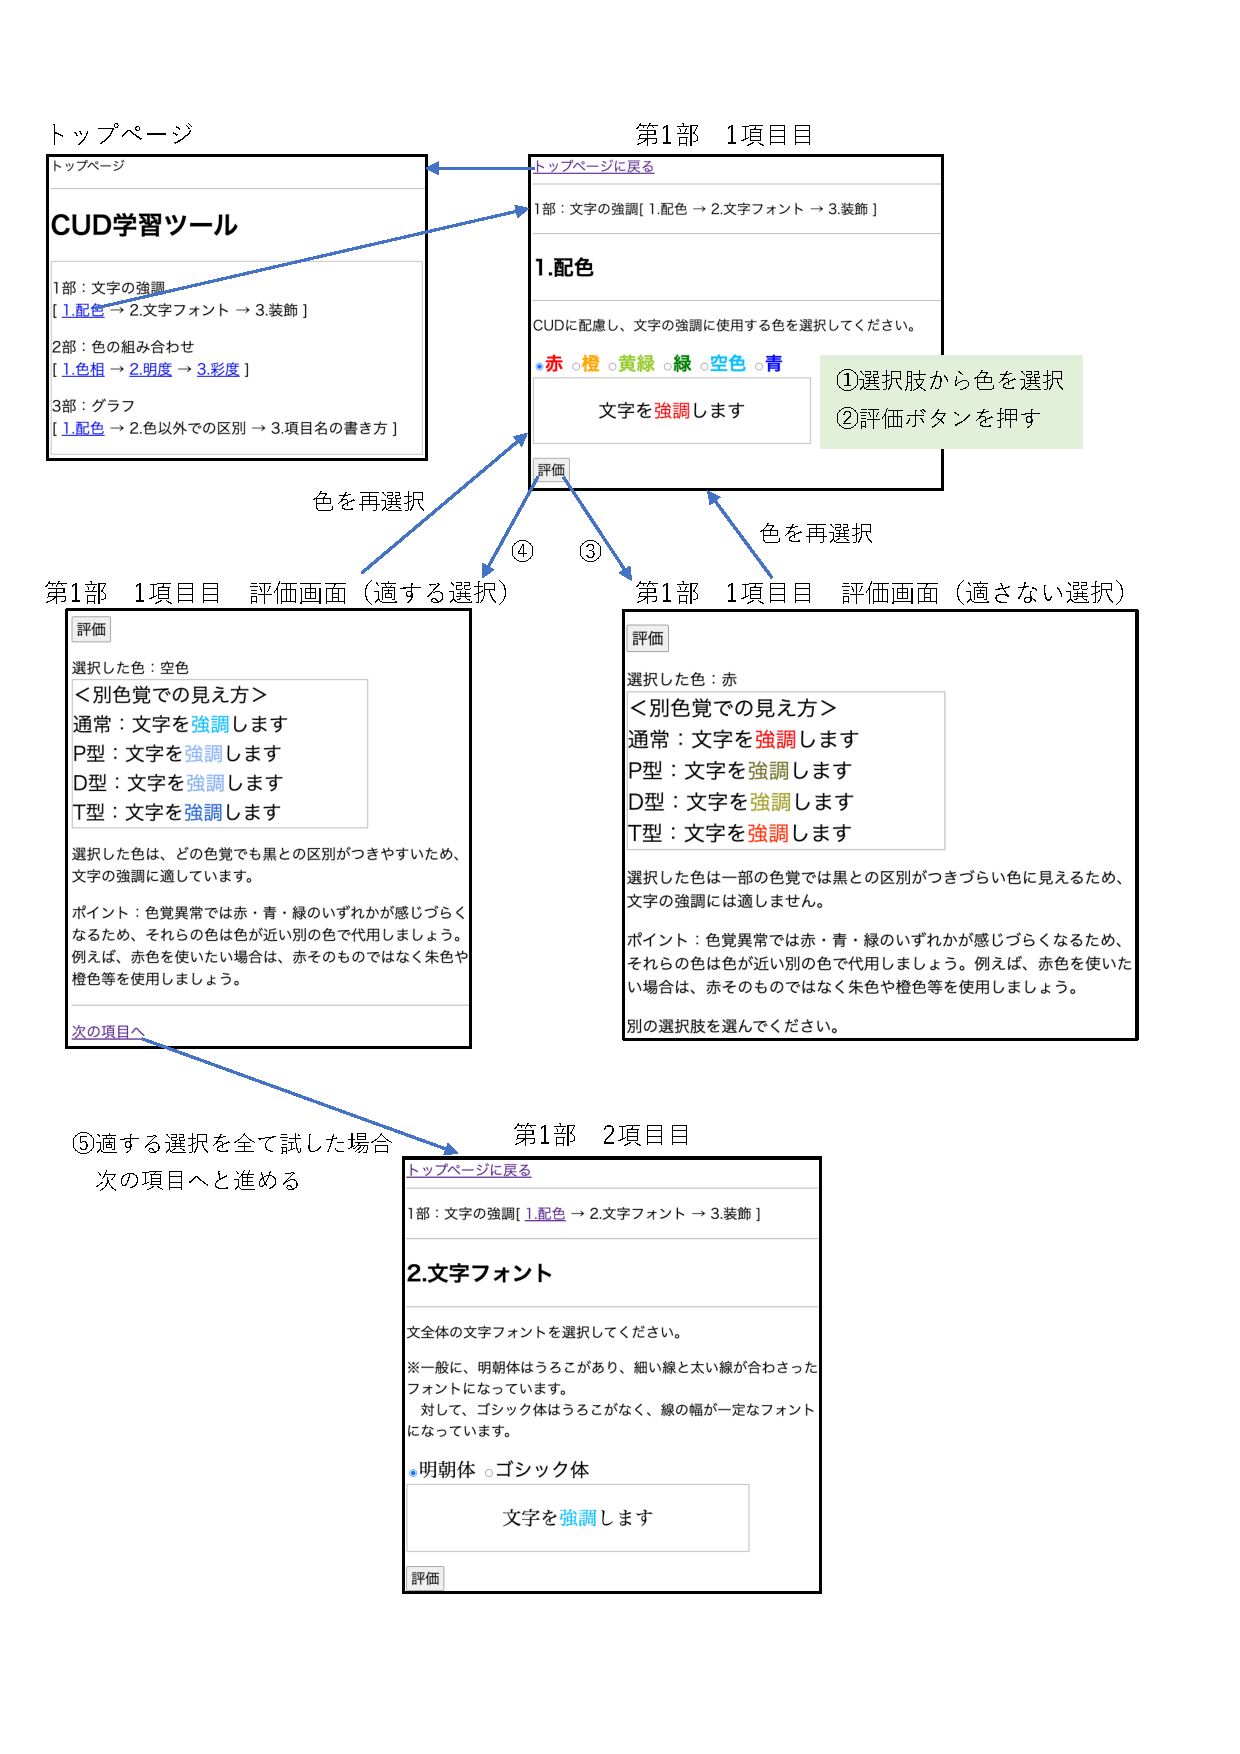
\includegraphics[clip,height=200mm]{images/map.pdf}
\end{center}
 \caption{サイトマップ}
 \label{fig:map}
\end{figure}

\clearpage

\subsection{学習ツールの構成}
本学習ツールは3部構成となっている.

\subsubsection{第1部 文字の強調}
1部では文字の強調を行う際の工夫について学習する.
項目として,配色,フォント,装飾の順に学習する.
図\ref{fig:gamen_1bu}は配色の学習画面である.

配色では,強調に使用する色を選択する.
選択肢は,赤,橙,黄緑,緑,空色,青の6種類である.
色覚異常は赤,青,緑のいずれかが感じづらくなるため,それらは黒との区別がつきづらい色に見える場合がある.
それらの色を選択した場合は文字の強調には適さないという評価とした.

フォントでは,選択肢から文全体のフォントを選択する.
選択肢は明朝体とゴシック体の2種類である.
明朝体には游明朝体やヒラギノ明朝等,複数の明朝体フォントが存在する.
これは,ゴシック体も同様である.
そのため,一概にどちらかが適さないフォントであると断定することは難しい.
一般に,明朝体はうろこがあり,細い線と太い線が合わさったフォントとなっている.
対して,ゴシック体はうろこがなく,線の幅が一定なフォントになっている.
そこでこの学習ツールでは,これらの特徴からCUDの観点で適しているか判断した.
線の一部が細くなっているフォントは色面積が小さくなり,色による判別がつきづらくなるため,色による文字の強調を行う際には適さないという評価とした.

装飾では,選択肢から選択することで,強調する文字を変化させる.
選択肢として,「アンダーラインを引く」と「太字にする」がある.
これらを選択することで,強調する文字を変化させる.
この項目では,色以外で強調を伝える方法を理解させることを目的としているため,これらの選択肢を選択して試した場合に,次の項目に進めるようにした.

\begin{figure}[h]
\begin{center}
 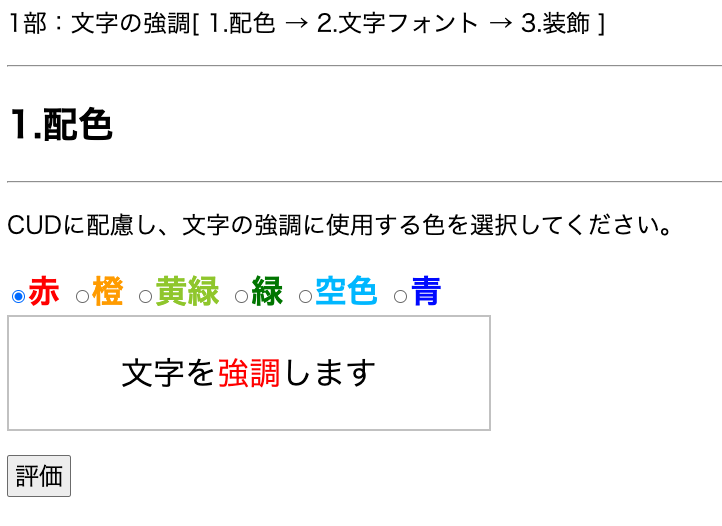
\includegraphics[clip,width=122mm,height=84mm]{images/gamen_1bu.png}
\end{center}
 \caption{1部の学習画面例}
 \label{fig:gamen_1bu}
\end{figure}

\clearpage
\subsubsection{第2部 色の組み合わせ}
2部では,色を組み合わせる際の工夫について学習する.
項目として,色相,明度,彩度の順に学習する.
図\ref{fig:gamen_2bu}は色相での学習画面である.
2部では,全ての項目で,指定された背景色に対する文字の色を選択するという学習の流れとなっており,選択肢が項目によって異なっている.
それぞれ扱っている色のうち1色が背景色となっており,それ以外が選択肢となっている.
背景色は「背景色を変更する」から変更することができる.

色相では,赤,橙,黄色,黄緑,緑,空色,青,紫の8種類を扱っている.
色相とは,赤,緑,青等の色味の種類のことである.
色相で別となっている2つの色の区別がつきづらい場合がある色覚が存在するため,別色覚での見え方を確認した際に,区別がつきづらい配色となる場合は適さないという評価とした.

明度では,明るめの橙,暗めの橙,明るめの緑,暗めの緑の4種類を扱っている.
明度とは,色の明るさのことである.
明度が高いほど白に近づき,低いほど黒に近くなる,
2色を組み合わせる場合は,明度に差をつけることで色覚によらず区別しやすい配色となるため,背景色と同じ明度の色を選択した場合は適さないという評価とした.

彩度では,赤,ピンク,青,水色の4種類を扱っている.
彩度とは,色の鮮やかさのことである.
彩度が高いほど明瞭な原色に近づき,低いほど白や黒等の無彩色に近づく.
彩度が低い色同士で組み合わせると,色による区別がつきづらい場合があるため,それらを組み合わせた場合は適さないという評価とした.

\begin{figure}[h]
\begin{center}
 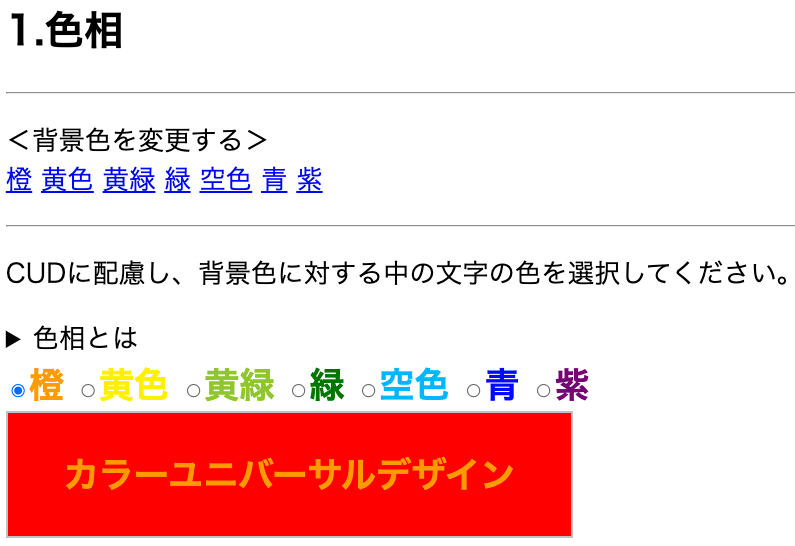
\includegraphics[clip,width=122mm,height=84mm]{images/gamen_2bu.png}
\end{center}
 \caption{2部の学習画面例}
 \label{fig:gamen_2bu}
\end{figure}


\clearpage
\subsubsection{第3部 グラフの作成}
3部では,グラフを作成する際の工夫について学習する.
この学習ツールでは,折れ線グラフを扱った.
項目として,線の色,色以外での区別,項目名の書き方の順に学習する.
図\ref{fig:gamen_3bu}は線の色での学習画面である.
線の色では,グラフに存在する3本の線の配色を選択する.
色の選択肢や配色に対する評価は,2部の1項目目である色相と同じである.

色以外での区別では,線の種類とマーカーの図形を選択する.
線の種類は,実線に加え間隔の異なる破線2種類の合計3種類を扱っている.
マーカーの図形は丸,三角,四角の3種類を扱っている.
線ごとに別々の組み合わせを用いることで,色に頼らず線の区別がつくようになる.
この学習ツールでは線の種類,マーカーの種類がそれぞれ3種類となっているため,それぞれで一つずつ選択していなかった場合は適さないという評価とした.

項目名の書き方では,項目名の表示方法を選択する.
選択肢は,「別枠にまとめる」と「線の近くに表示する」の2種類である.
項目名は,別枠にまとめて表示するのではなく,それぞれの線の近くに表示することで,色に頼らなくとも項目名と線の対応が伝わるようになる.
そのため「別枠にまとめる」を選択した場合は適さないという評価とした.

\begin{figure}[h]
\begin{center}
 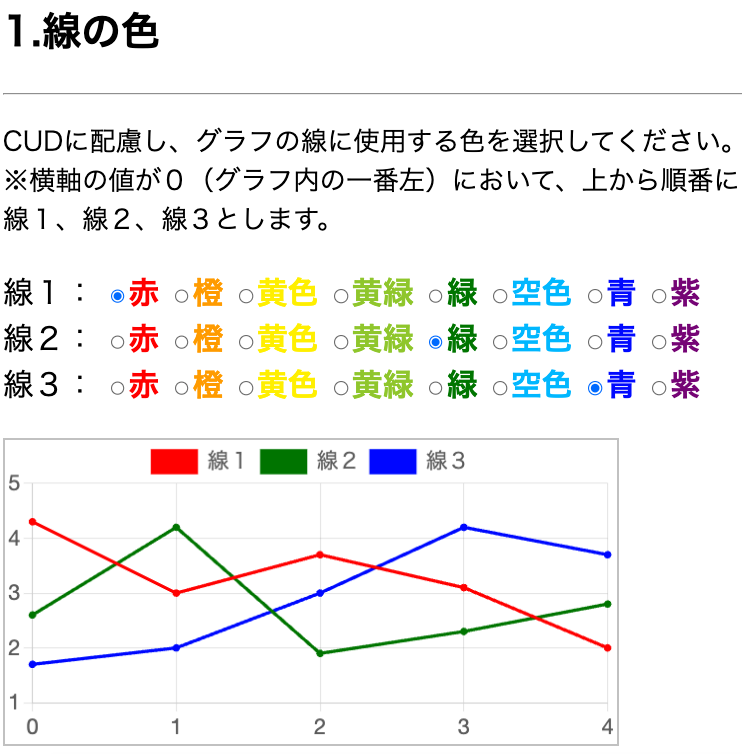
\includegraphics[clip,width=93mm,height=94mm]{images/gamen_3bu.png}
\end{center}
 \caption{3部の学習画面例}
 \label{fig:gamen_3bu}
\end{figure}
